\section{An Automaton-Theoretic Representation of DDTs}
\label{sec:automaton}

The presents a novel DDT representation using automaton theory based on the hypothesis that the derivative of functions used as S-boxes in popular ciphers are not random, but possess significant structural regularities that can be exploited for compression. We first point the fundamental limitations of representing the DDT as a dense matrix and then introduce a representation, showing the process to convert a DDT into an automaton using less storage.

\subsection{Structural Redundancy in DDTs}
\label{sec:redundancies}

For an $n$-bit S-box, the representation of its DDT as a matrix requires $2^{2n}$ elements, which quickly becomes prohibitive for storage, and in-memory analysis as $n$ increases. The inefficiency of this representation is the result of two types of redundancy. The first is the general redundancy present in every DDT: because the number of distinct differential values is significantly smaller than the total number of cells, many cells have the same value. For instance, at least half of the DDT entries are always zero. The second is the specific redundancy resulting from the properties of the S-box, which manifests as the frequent repetition of small, identical patterns or blocks throughout the table.

This specific redundancy is particularly visible in the DDT of the PRESENT S-box, as illustrated in Table~\ref{tab:present_ddt_blocks}. In this visualization, the table is partitioned into $2 \times 2$ blocks, and colors are assigned to each according to its frequency: higher frequency of blocks receive darker colors while less frequent blocks receive lighter ones. In this particular case, 25 out of 64 blocks in the table falls into only 3 block patterns, with the all-zero block having 11 occurrences. This provides a hint that we can use the same structure to represent a significant portion of the DDT.

\begin{table}
    \caption{The DDT of the PRESENT S-box, partitioned into 2×2 blocks. Blocks with the same frequency share the same color.}
    \label{tab:present_ddt_blocks}
    
    \centering

    \begin{tabular}{|*{8}{w{c}{0.03\textwidth}w{c}{0.03\textwidth}|}}

        \hline
        
        \cellcolor{Color6}\textcolor{Gelo}0 &
        \cellcolor{Color6}\textcolor{Gelo}0 &
        \cellcolor{Color4}0 & \cellcolor{Color4}0 & 
        \cellcolor{Color6}\textcolor{Gelo}0 & \cellcolor{Color6}\textcolor{Gelo}0 & 
        \cellcolor{Color4}0 & \cellcolor{Color4}0 &
        \cellcolor{Color4}0 & \cellcolor{Color4}0 & 
        \cellcolor{Color6}\textcolor{Gelo}0 & \cellcolor{Color6}\textcolor{Gelo}0 &
        \cellcolor{Color4}0 & \cellcolor{Color4}0 & \cellcolor{Color6}\textcolor{Gelo}0 & \cellcolor{Color6}\textcolor{Gelo}0 \\
        
        \cellcolor{Color6}\textcolor{Gelo}0 & \cellcolor{Color6}\textcolor{Gelo}0 &
        \cellcolor{Color4}0 & \cellcolor{Color4}4 & \cellcolor{Color6}\textcolor{Gelo}0 & \cellcolor{Color6}\textcolor{Gelo}0 &
        \cellcolor{Color4}0 & \cellcolor{Color4}4 &
        \cellcolor{Color4}0 & \cellcolor{Color4}4 & \cellcolor{Color6}\textcolor{Gelo}0 & \cellcolor{Color6}\textcolor{Gelo}0 &
        \cellcolor{Color4}0 & \cellcolor{Color4}4 & \cellcolor{Color6}\textcolor{Gelo}0 & \cellcolor{Color6}\textcolor{Gelo}0 \\
        
        \hline
        
        \cellcolor{Color3}0 & \cellcolor{Color3}0 & \cellcolor{Color3}0 & \cellcolor{Color3}2 & \cellcolor{Color3}0 & \cellcolor{Color3}4 & \cellcolor{Color3}2 & \cellcolor{Color3}0 & \cellcolor{Color6}\textcolor{Gelo}0 & \cellcolor{Color6}\textcolor{Gelo}0 &
        \cellcolor{Color3}2 & \cellcolor{Color3}0 & \cellcolor{Color5}2 & \cellcolor{Color5}2 &
        \cellcolor{Color3}2 & \cellcolor{Color3}0 \\
        
        \cellcolor{Color3}0 & \cellcolor{Color3}2 & \cellcolor{Color3}0 & \cellcolor{Color3}2 & \cellcolor{Color3}2 & \cellcolor{Color3}0 & \cellcolor{Color3}4 & \cellcolor{Color3}2 & \cellcolor{Color6}\textcolor{Gelo}0 & \cellcolor{Color6}\textcolor{Gelo}0 &
        \cellcolor{Color3}2 & \cellcolor{Color3}2 & \cellcolor{Color5}0 & \cellcolor{Color5}0 &
        \cellcolor{Color3}0 & \cellcolor{Color3}0 \\
        
        \hline
        
        \cellcolor{Color3}0 & \cellcolor{Color3}0 & \cellcolor{Color6}\textcolor{Gelo}0 & \cellcolor{Color6}\textcolor{Gelo}0 &
        \cellcolor{Color3}0 & \cellcolor{Color3}4 & \cellcolor{Color5}2 & \cellcolor{Color5}2 &
        \cellcolor{Color3}0 & \cellcolor{Color3}2 & \cellcolor{Color3}2 & \cellcolor{Color3}0 & \cellcolor{Color3}2 & \cellcolor{Color3}0 & \cellcolor{Color3}2 & \cellcolor{Color3}0 \\
        
        \cellcolor{Color3}0 & \cellcolor{Color3}2 & \cellcolor{Color6}\textcolor{Gelo}0 & \cellcolor{Color6}\textcolor{Gelo}0 &
        \cellcolor{Color3}2 & \cellcolor{Color3}0 & \cellcolor{Color5}0 & \cellcolor{Color5}0 &
        \cellcolor{Color3}0 & \cellcolor{Color3}2 & \cellcolor{Color3}2 & \cellcolor{Color3}2 & \cellcolor{Color3}4 & \cellcolor{Color3}2 & \cellcolor{Color3}0 & \cellcolor{Color3}0 \\ 
        
        \hline
        
        \cellcolor{Color4}0 & \cellcolor{Color4}0 &
        \cellcolor{Color3}2 & \cellcolor{Color3}0 & \cellcolor{Color6}\textcolor{Gelo}0 & \cellcolor{Color6}\textcolor{Gelo}0 &
        \cellcolor{Color3}2 & \cellcolor{Color3}0 & \cellcolor{Color3}2 & \cellcolor{Color3}0 & \cellcolor{Color2}0 & \cellcolor{Color2}4 & \cellcolor{Color3}2 & \cellcolor{Color3}0 &
        \cellcolor{Color1}0 & \cellcolor{Color1}4 \\
        
        \cellcolor{Color4}0 & \cellcolor{Color4}4 &
        \cellcolor{Color3}2 & \cellcolor{Color3}0 & \cellcolor{Color6}\textcolor{Gelo}0 & \cellcolor{Color6}\textcolor{Gelo}0 &
        \cellcolor{Color3}2 & \cellcolor{Color3}0 & \cellcolor{Color3}2 & \cellcolor{Color3}0 & \cellcolor{Color2}0 & \cellcolor{Color2}0 & \cellcolor{Color3}2 & \cellcolor{Color3}0 &
        \cellcolor{Color1}0 & \cellcolor{Color1}4 \\
        
        \hline
        
        \cellcolor{Color6}\textcolor{Gelo}0 & \cellcolor{Color6}\textcolor{Gelo}0 &
        \cellcolor{Color3}0 & \cellcolor{Color3}2 & \cellcolor{Color2}0 & \cellcolor{Color2}0 & \cellcolor{Color3}0 & \cellcolor{Color3}2 & \cellcolor{Color3}0 & \cellcolor{Color3}2 & \cellcolor{Color2}0 & \cellcolor{Color2}4 & \cellcolor{Color3}0 & \cellcolor{Color3}2 &
        \cellcolor{Color1}0 & \cellcolor{Color1}4 \\
        
        \cellcolor{Color6}\textcolor{Gelo}0 & \cellcolor{Color6}\textcolor{Gelo}0 &
        \cellcolor{Color3}2 & \cellcolor{Color3}0 & \cellcolor{Color2}4 & \cellcolor{Color2}0 & \cellcolor{Color3}2 & \cellcolor{Color3}0 & \cellcolor{Color3}2 & \cellcolor{Color3}0 & \cellcolor{Color2}0 & \cellcolor{Color2}0 & \cellcolor{Color3}2 & \cellcolor{Color3}0 &
        \cellcolor{Color1}4 & \cellcolor{Color1}0 \\
        
        \hline
        
        \cellcolor{Color3}0 & \cellcolor{Color3}0 & \cellcolor{Color5}2 & \cellcolor{Color5}2 &
        \cellcolor{Color3}0 & \cellcolor{Color3}4 & \cellcolor{Color6}\textcolor{Gelo}0 & \cellcolor{Color6}\textcolor{Gelo}0 &
        \cellcolor{Color3}2 & \cellcolor{Color3}0 & \cellcolor{Color3}2 & \cellcolor{Color3}0 & \cellcolor{Color3}0 & \cellcolor{Color3}2 & \cellcolor{Color3}2 & \cellcolor{Color3}0 \\
        
        \cellcolor{Color3}0 & \cellcolor{Color3}2 & \cellcolor{Color5}0 & \cellcolor{Color5}0 &
        \cellcolor{Color3}2 & \cellcolor{Color3}0 & \cellcolor{Color6}\textcolor{Gelo}0 & \cellcolor{Color6}\textcolor{Gelo}0 &
        \cellcolor{Color3}4 & \cellcolor{Color3}2 & \cellcolor{Color3}2 & \cellcolor{Color3}2 & \cellcolor{Color3}0 & \cellcolor{Color3}2 & \cellcolor{Color3}0 & \cellcolor{Color3}0 \\
        
        \hline
        
        \cellcolor{Color3}0 & \cellcolor{Color3}0 & \cellcolor{Color3}2 & \cellcolor{Color3}0 & \cellcolor{Color3}0 & \cellcolor{Color3}4 & \cellcolor{Color3}0 & \cellcolor{Color3}2 & \cellcolor{Color5}2 & \cellcolor{Color5}2 &
        \cellcolor{Color3}2 & \cellcolor{Color3}0 & \cellcolor{Color6}\textcolor{Gelo}0 & \cellcolor{Color6}\textcolor{Gelo}0 &
        \cellcolor{Color3}2 & \cellcolor{Color3}0 \\
        
        \cellcolor{Color3}0 & \cellcolor{Color3}2 & \cellcolor{Color3}4 & \cellcolor{Color3}2 & \cellcolor{Color3}2 & \cellcolor{Color3}0 & \cellcolor{Color3}0 & \cellcolor{Color3}2 & \cellcolor{Color5}0 & \cellcolor{Color5}0 &
        \cellcolor{Color3}2 & \cellcolor{Color3}2 & \cellcolor{Color6}\textcolor{Gelo}0 & \cellcolor{Color6}\textcolor{Gelo}0 &
        \cellcolor{Color3}0 & \cellcolor{Color3}0 \\
        
        \hline
        
        \cellcolor{Color4}0 & \cellcolor{Color4}0 & \cellcolor{Color5}2 & \cellcolor{Color5}2 &
        \cellcolor{Color2}0 & \cellcolor{Color2}0 & \cellcolor{Color5}2 & \cellcolor{Color5}2 &
        \cellcolor{Color5}2 & \cellcolor{Color5}2 &
        \cellcolor{Color6}\textcolor{Gelo}0 & \cellcolor{Color6}\textcolor{Gelo}0 &
        \cellcolor{Color5}2 & \cellcolor{Color5}2 &
        \cellcolor{Color1}0 & \cellcolor{Color1}0 \\
         
        \cellcolor{Color4}0 & \cellcolor{Color4}4 & \cellcolor{Color5}0 & \cellcolor{Color5}0 &
        \cellcolor{Color2}4 & \cellcolor{Color2}0 & \cellcolor{Color5}0 & \cellcolor{Color5}0 &
        \cellcolor{Color5}0 & \cellcolor{Color5}0 &
        \cellcolor{Color6}\textcolor{Gelo}0 & \cellcolor{Color6}\textcolor{Gelo}0 &
        \cellcolor{Color5}0 & \cellcolor{Color5}0 &
        \cellcolor{Color1}4 & \cellcolor{Color1}4 \\
        
        \hline
    
    \end{tabular}

    \vspace{0.25em}

    \begin{center}
    \footnotesize
    \textbf{Legend} \par

    \begin{tabular}{*{3}{w{c}{0.03\textwidth}rl}}
         \\

         \cellcolor{Color6} & \ 11 & occurrences \ &
         \cellcolor{Color5}\phantom{XX} & \ 8 & occurrences \ &
         \cellcolor{Color4}\phantom{XX} & \ 6 & occurrences \\
         \cellcolor{Color3}\phantom{XX} & \ 4 & occurrences \ &
         \cellcolor{Color2}\phantom{XX} & \ 2 & occurrences \ &
         \cellcolor{Color1}\phantom{XX} & \ 1 & occurrence \\
    \end{tabular}
    \end{center}
\end{table}


To capture both general and specific regularities of DDTs, we propose a method that reframes these tables as formal languages and represents them using finite automata. This approach draws from techniques used in image compression and Boolean functions representation and provides a canonical and compressed representation of a DDT.

\subsection{Constructing a finite automaton from a DDT}

To transform a DDT into a finite automaton, we employ techniques established in \cite{BerstelAndMorcrette} and \cite{BerstelAndNaitAbdallah}. Let $\Sigma = \{0, 1, 2, 3\}$ be a quaternary alphabet. We assign the whole matrix the empty string $\varepsilon$. Then, we partition the $2^{n} \times 2^{n}$ DDT matrix into four equal $2^{n - 1} \times 2^{n - 1}$ quadrants, assigning a distinct symbol from $\Sigma$ to each. This partitioning is applied recursively, subdividing each subsequent sub-matrix. If a sub-matrix is assigned the string $w$, its four quadrants are assigned strings $wa$ for each $a$ in $\Sigma$. This process continues until reaching the individual cells that represent the differential uniformity values. Consequently, the coordinates of each cell in the DDT are mapped to a set of strings S. The subset of $S$ comprising strings that correspond to non-zero entries of the DDT we call the language of the DDT, and denote by $L(DDT)$. Figure~\ref{fig:encoding_example} illustrates this recursive assigning scheme in detail for an $8 \times 8$ DDT. In (a), the initial DDT is first partitioned into four primary quadrants, each represented by a single symbol from $\Sigma$. This recursive subdivision is demonstrated further in (b), where each sub-quadrant is assigned a string of length two by appending symbols to the string of its containing quadrant. This partitioning reaches the individual cell level in (c), where the highlighted cell is uniquely encoded by the string \texttt{320}."

\begin{figure}
    \caption{Recursive quadrant encoding of an $8 \times 8$ DDT. Item (a) shows the whole table divided into 4 quadrants; Item (b) shows each quadrant further divided into 4 subquadrants; Item (c) highlights the cell encoded as \texttt{320}.}
    \label{fig:encoding_example}

    \centering

    \vspace{1em}

    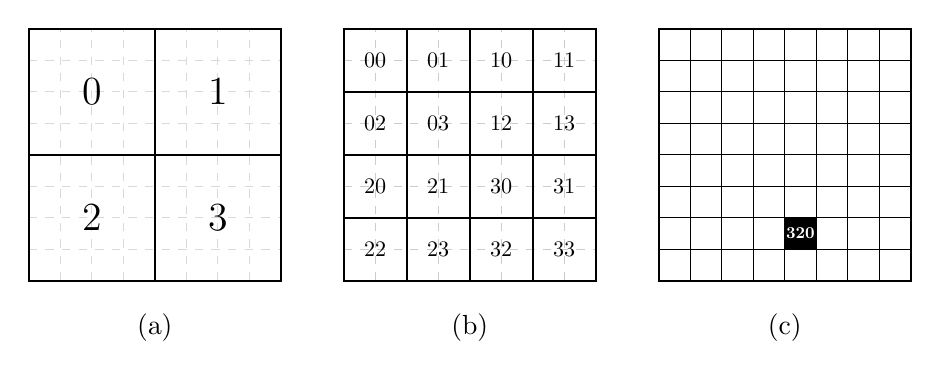
\begin{tikzpicture}[scale=0.4]
        \begin{scope}[shift={(0,0)}]
            \draw[step=1, gray!30, thin, dashed] (0,0) grid (8,8);
            \draw[thick] (0,0) rectangle (8,8);
            \draw[thick] (4,0) -- (4,8);
            \draw[thick] (0,4) -- (8,4);
            
            \node at (2,6) {\Large 0};
            \node at (6,6) {\Large 1};
            \node at (2,2) {\Large 2};
            \node at (6,2) {\Large 3};
            \node at (4,-1.5) {\normalsize (a)};
        \end{scope}

        \begin{scope}[shift={(10,0)}]
            \draw[step=1, gray!40, thin, dashed] (0,0) grid (8,8);
            \draw[thick] (0,0) rectangle (8,8);
            \draw[thick] (4,0) -- (4,8);
            \draw[thick] (0,4) -- (8,4);
            \draw[thick] (2,0) -- (2,8); \draw[thick] (6,0) -- (6,8);
            \draw[thick] (0,2) -- (8,2); \draw[thick] (0,6) -- (8,6);

            \foreach \x/\y/\label in {1/7/00, 3/7/01, 1/5/02, 3/5/03, 5/7/10, 7/7/11, 5/5/12, 7/5/13, 1/3/20, 3/3/21, 1/1/22, 3/1/23, 5/3/30, 7/3/31, 5/1/32, 7/1/33} {
                \node[scale=0.8] at (\x,\y) {\normalsize \label};
            }
            \node at (4,-1.5) {\normalsize (b)};
        \end{scope}

        \begin{scope}[shift={(20,0)}]
            \draw[step=1, thin] (0,0) grid (8,8);
            \draw[thick] (0,0) rectangle (8,8);
            
            \fill[black] (4,1) rectangle (5,2); 
            \node[scale=0.6, text=white, font=\bfseries] at (4.5,1.5) {320};
            \node at (4,-1.5) {\normalsize (c)};
        \end{scope}
    \end{tikzpicture}
\end{figure}






% \begin{table}[ht]
%     \caption{Recursive quadrant encoding representations.}
%     \label{tab:encoding_example}
%     \centering
%     \renewcommand{\arraystretch}{1.0}
%     \setlength{\tabcolsep}{4pt}
%     \begin{tabular}{c@{\hskip 0.3in}c@{\hskip 0.3in}c}
%         \begin{tabular}{|*{8}{c|}}
%         \hline
%         ~ & ~ & ~ & ~ & ~ & ~ & ~ & ~ \\ \hline
%         ~ & ~ & ~ & ~ & ~ & ~ & ~ & ~ \\ \hline
%         ~ & ~ & ~ & ~ & ~ & ~ & ~ & ~ \\ \hline
%         ~ & ~ & ~ & ~ & ~ & ~ & ~ & ~ \\ \hline
%         ~ & ~ & ~ & ~ & ~ & ~ & ~ & ~ \\ \hline
%         ~ & ~ & ~ & ~ & ~ & ~ & ~ & ~ \\ \hline
%         ~ & ~ & ~ & ~ & ~ & ~ & ~ & ~ \\ \hline
%         ~ & ~ & ~ & ~ & ~ & ~ & ~ & ~ \\ \hline
%         \end{tabular}
%         &
%         \begin{tabular}{|*{8}{c|}}
%         \hline
%         ~ & ~ & ~ & ~ & ~ & ~ & ~ & ~ \\ \hline
%         ~ & ~ & ~ & ~ & ~ & ~ & ~ & ~ \\ \hline
%         ~ & ~ & ~ & ~ & ~ & ~ & ~ & ~ \\ \hline
%         ~ & ~ & ~ & ~ & ~ & ~ & ~ & ~ \\ \hline
%         ~ & ~ & ~ & ~ & ~ & ~ & ~ & ~ \\ \hline
%         ~ & ~ & ~ & ~ & ~ & ~ & ~ & ~ \\ \hline
%         ~ & ~ & ~ & ~ & ~ & ~ & ~ & ~ \\ \hline
%         ~ & ~ & ~ & ~ & ~ & ~ & ~ & ~ \\ \hline
%         \end{tabular}
%         &
%         \begin{tabular}{|*{8}{c|}}
%         \hline
%         ~ & ~ & ~ & ~ & ~ & ~ & ~ & ~ \\ \hline
%         ~ & ~ & ~ & ~ & ~ & ~ & ~ & ~ \\ \hline
%         ~ & ~ & ~ & ~ & ~ & ~ & ~ & ~ \\ \hline
%         ~ & ~ & ~ & ~ & ~ & ~ & ~ & ~ \\ \hline
%         ~ & ~ & ~ & ~ & ~ & ~ & ~ & ~ \\ \hline
%         ~ & ~ & ~ & ~ & ~ & ~ & ~ & ~ \\ \hline
%         ~ & ~ & ~ & ~ & ~ & ~ & ~ & ~ \\ \hline
%         ~ & ~ & ~ & ~ & ~ & ~ & ~ & ~ \\ \hline
%         \end{tabular} \\
%         (a) & (b) & (c)
%     \end{tabular}
% \end{table}



% \begin{table}
%     \caption{Recursive quadrant encoding for a $8 \times 8$ DDT. Each cell is uniquely identified by a 4-symbol word. For example, the highlighted region corresponds to all words with the prefix \texttt{320}.}
%     \label{tab:encoding_example}
    
%     \centering
%     \renewcommand{\arraystretch}{1.4}
%     \ttfamily
    
%     \begin{tabular}{|*{16}{C{0.08\textwidth}|}}
    
%     \hline

%     \multicolumn{8}{|C{0.32\textwidth}|}{\multirow{8}{*}{\Huge 0}} & \multicolumn{4}{C{0.16\textwidth}|}{\multirow{4}{*}{\Large 10}} & \multicolumn{4}{C{0.16\textwidth}|}{\multirow{4}{*}{\Large 11}} \\
%     \multicolumn{8}{|C{0.08\textwidth}|}{}                         & \multicolumn{4}{C{0.08\textwidth}|}{}                           & \multicolumn{4}{C{0.08\textwidth}|}{}                           \\
%     \multicolumn{8}{|C{0.08\textwidth}|}{}                         & \multicolumn{4}{C{0.08\textwidth}|}{}                           & \multicolumn{4}{C{0.08\textwidth}|}{}                           \\
%     \multicolumn{8}{|C{0.08\textwidth}|}{}                         & \multicolumn{4}{C{0.08\textwidth}|}{}                           & \multicolumn{4}{C{0.08\textwidth}|}{}                           \\
    
%     \cline{9-16}
    
%     \multicolumn{8}{|C{0.08\textwidth}|}{}                         & \multicolumn{4}{C{0.16\textwidth}|}{\multirow{4}{*}{\Large 12}} & \multicolumn{4}{C{0.16\textwidth}|}{\multirow{4}{*}{\Large 13}} \\
%     \multicolumn{8}{|C{0.08\textwidth}|}{}                         & \multicolumn{4}{C{0.08\textwidth}|}{}                           & \multicolumn{4}{C{0.08\textwidth}|}{}                           \\
%     \multicolumn{8}{|C{0.08\textwidth}|}{}                         & \multicolumn{4}{C{0.08\textwidth}|}{}                           & \multicolumn{4}{C{0.08\textwidth}|}{}                           \\
%     \multicolumn{8}{|C{0.08\textwidth}|}{}                         & \multicolumn{4}{C{0.08\textwidth}|}{}                           & \multicolumn{4}{C{0.08\textwidth}|}{}                           \\
    
%     \hline
    
%     \multicolumn{2}{|C{0.08\textwidth}|}{\multirow{2}{*}{200}} & \multicolumn{2}{C{0.08\textwidth}|}{\multirow{2}{*}{201}} & \multicolumn{2}{C{0.08\textwidth}|}{\multirow{2}{*}{210}} & \multicolumn{2}{C{0.08\textwidth}|}{\multirow{2}{*}{211}} & \multicolumn{2}{C{0.08\textwidth}|}{\multirow{2}{*}{300}}  & \multicolumn{2}{C{0.08\textwidth}|}{\multirow{2}{*}{301}} & \multicolumn{2}{C{0.08\textwidth}|}{\multirow{2}{*}{310}} & \multicolumn{2}{C{0.08\textwidth}|}{\multirow{2}{*}{311}} \\
    
%     \multicolumn{2}{|C{0.08\textwidth}|}{}                     & \multicolumn{2}{C{0.08\textwidth}|}{}                     & \multicolumn{2}{C{0.08\textwidth}|}{}                     & \multicolumn{2}{C{0.08\textwidth}|}{}                     & \multicolumn{2}{C{0.08\textwidth}|}{}                      & \multicolumn{2}{C{0.08\textwidth}|}{}                     & \multicolumn{2}{C{0.08\textwidth}|}{}                         & \multicolumn{2}{C{0.08\textwidth}|}{}                     \\ 
    
%     \cline{1-16}
    
%     % Row 11-12: Sub-quadrants 20 and 21 (left), 30 and 31 (right)
%     \multicolumn{2}{|C{0.08\textwidth}|}{\multirow{2}{*}{202}} & \multicolumn{2}{C{0.08\textwidth}|}{\multirow{2}{*}{203}} & \multicolumn{2}{C{0.08\textwidth}|}{\multirow{2}{*}{212}} & \multicolumn{2}{C{0.08\textwidth}|}{\multirow{2}{*}{213}} & \multicolumn{2}{C{0.08\textwidth}|}{\multirow{2}{*}{302}}  & \multicolumn{2}{C{0.08\textwidth}|}{\multirow{2}{*}{303}} & \multicolumn{2}{C{0.08\textwidth}|}{\multirow{2}{*}{312}} & \multicolumn{2}{C{0.08\textwidth}|}{\multirow{2}{*}{313}} \\
    
%     \multicolumn{2}{|C{0.08\textwidth}|}{}                     & \multicolumn{2}{C{0.08\textwidth}|}{}                     & \multicolumn{2}{C{0.08\textwidth}|}{}                     & \multicolumn{2}{C{0.08\textwidth}|}{}                     & \multicolumn{2}{C{0.08\textwidth}|}{}                      & \multicolumn{2}{C{0.08\textwidth}|}{}                     & \multicolumn{2}{C{0.08\textwidth}|}{}                         & \multicolumn{2}{C{0.08\textwidth}|}{}                     \\
    
%     \hline
    
%     % Row 13-14: Sub-quadrants 22 and 23 (left), 32 and 33 (right)
%     \multicolumn{2}{|C{0.08\textwidth}|}{\multirow{2}{*}{220}}  & \multicolumn{2}{C{0.08\textwidth}|}{\multirow{2}{*}{221}} & \multicolumn{2}{C{0.08\textwidth}|}{\multirow{2}{*}{230}} & \multicolumn{2}{C{0.08\textwidth}|}{\multirow{2}{*}{231}} & \multicolumn{2}{C{0.08\textwidth}|}{\cellcolor{Color1}\multirow{2}{*}{320}} & \multicolumn{2}{C{0.08\textwidth}|}{\multirow{2}{*}{321}} & \multicolumn{2}{C{0.08\textwidth}|}{\multirow{2}{*}{330}} & \multicolumn{2}{C{0.08\textwidth}|}{\multirow{2}{*}{331}} \\
    
%     \multicolumn{2}{|C{0.08\textwidth}|}{}                      & \multicolumn{2}{C{0.08\textwidth}|}{}                     & \multicolumn{2}{C{0.08\textwidth}|}{}                     & \multicolumn{2}{C{0.08\textwidth}|}{}                     & \multicolumn{2}{C{0.08\textwidth}|}{\cellcolor{Color1}\multirow{-2}{*}{320}}                     & \multicolumn{2}{C{0.08\textwidth}|}{}                     & \multicolumn{2}{C{0.08\textwidth}|}{}                     & \multicolumn{2}{C{0.08\textwidth}|}{}                     \\
    
%     \cline{1-16}
    
%     % Row 15-16: Sub-quadrants 22 and 23 (left), 32 and 33 (right)
%     \multicolumn{2}{|C{0.08\textwidth}|}{\multirow{2}{*}{222}} & \multicolumn{2}{C{0.08\textwidth}|}{\multirow{2}{*}{223}} & \multicolumn{2}{C{0.08\textwidth}|}{\multirow{2}{*}{232}} & \multicolumn{2}{C{0.08\textwidth}|}{\multirow{2}{*}{233}} & \multicolumn{2}{C{0.08\textwidth}|}{\multirow{2}{*}{322}} & \multicolumn{2}{C{0.08\textwidth}|}{\multirow{2}{*}{323}} & \multicolumn{2}{C{0.08\textwidth}|}{\multirow{2}{*}{332}} & \multicolumn{2}{C{0.08\textwidth}|}{\multirow{2}{*}{333}} \\
    
%     \multicolumn{2}{|C{0.08\textwidth}|}{}                     & \multicolumn{2}{C{0.08\textwidth}|}{}                     & \multicolumn{2}{C{0.08\textwidth}|}{}                     & \multicolumn{2}{C{0.08\textwidth}|}{}                     & \multicolumn{2}{C{0.08\textwidth}|}{}                     & \multicolumn{2}{C{0.08\textwidth}|}{}                     & \multicolumn{2}{C{0.08\textwidth}|}{}                          & \multicolumn{2}{C{0.08\textwidth}|}{}                     \\
    
%     \hline
    
%     \end{tabular}
% \end{table}


Following the structural mapping, $L(DDT)$ is represented by a quaternary finite automaton where each path from the initial state to a terminal state corresponds to a word $w \in \Sigma^{n}$. In this construction, the internal states represent the sub-matrices generated during the recursive partition, while the transitions are dictated by the symbols of the alphabet $\Sigma$. Unlike standard finite automata, which only outputs 0 or 1 to either accept or reject, this automaton must output the values in the DDT. To achieve this, we define a function $f_{D} : \Sigma^{n} \to \mathbb{N}$. Consequently, the evaluation of any word $w \in \Sigma^{n}$ not only verifies if the corresponding differential is possible but also returns its number of occurrences.

To optimize storage, minimization is necessary. But since standard automata evaluate to 0 or 1 only, classical minimization algorithms cannot be directly applied; otherwise, they would merge accept states that refer to different values in the DDT. Specifically, we draw upon the relationship between finite automata and decision diagrams \cite{KimuraAndClarke1990} and multi-terminal binary decision diagrams, which extend standard binary decision diagrams by allowing arbitrary integer terminals \cite{FujitaEtAl1997}. By combining these concepts, we create a quaternary variant of a multi-terminal decision diagram to represent and minimize our automaton.

The compression process corresponds directly to the reductions of this decision diagram, which is achieved by eliminating redundant vertices and duplicate subgraphs. Because our alphabet contains four symbols, we modify traditional binary decision diagrams \cite{Bryant1986} to accommodate our quaternary format. First, each internal node $v$ possesses four children instead of two, denoted $E_{i}(v)$ for $1 \leq i \leq 4$. Second, we modify two rules used to assign a repeated identifier to a node $v$, deeming it redundant:

\begin{enumerate}
    \item If all of its four children have the same identifier, that is, $id(E_{i}(v)) = id(E_{j}(v))$ for all $1 \leq i < j \leq 4$, we set $id(v) = id(E_{1}(v))$.
    
    \item If there exists a node $u$ such that the corresponding children of $u$ and $v$ have the same identifier, that is, $id(E_{i}(u)) = id(E_{i}(v))$ for all $1 \leq i \leq 4$, we set $id(v) = id(u)$.
\end{enumerate}

Given the equivalence between finite automata and decision diagrams, applying these reduction rules yields a compressed structure. While the resulting finite automaton is not minimal in the standard sense, it is minimal and canonical within our context. The final step of the compression is to remove the strings corresponding to redundant accept states from the function table. This leaves exactly one entry for each distinct value present in the DDT.

To illustrate this construction and minimization process, we use the 3-bit S-box of the SEA cipher. The corresponding DDT is shown in Table~\ref{tbl:sea-ddt}. Because this S-box is an APN function, its only possible non-zero differential value is 2. Note that the trivial differential at coordinate $(0,0)$ is treated as having a value of 0, rather than $2^{3}$. Since this transition is irrelevant for differential cryptanalysis, overriding its value increases the sparsity of the matrix and optimizes the resulting automaton.

\begin{table}[!ht]
    \label{tbl:sea-ddt}
    \caption{DDT for the 3-bit S-box used in the SEA cipher.}
    
    \centering
    \scriptsize
    \renewcommand{\arraystretch}{1.5}

    \begin{tabular}{c|*{8}{C{0.04\textwidth}}}
        \diagbox{\phantom{X}$\alpha$}{$\beta$\phantom{X}} & 000 & 001 & 010 & 011 & 100 & 101 & 110 & 111 \\ \hline
        000 & 0 & 0 & 0 & 0 & 0 & 0 & 0 & 0 \\
        001 & 0 & 2 & 0 & 2 & 0 & 2 & 0 & 2 \\
        010 & 0 & 2 & 2 & 0 & 0 & 2 & 2 & 0 \\
        011 & 0 & 0 & 2 & 2 & 0 & 0 & 2 & 2 \\
        100 & 0 & 0 & 0 & 0 & 2 & 2 & 2 & 2 \\
        101 & 0 & 2 & 0 & 2 & 2 & 0 & 2 & 0 \\
        110 & 0 & 2 & 2 & 0 & 2 & 0 & 0 & 2 \\
        111 & 0 & 0 & 2 & 2 & 2 & 2 & 0 & 0 \\
    \end{tabular}
\end{table}

Following the structural mapping, the uncompressed quaternary finite automaton representing this DDT is depicted in Figure~\ref{fig:sea-automaton}. This initial automaton explicitly encodes all 28 valid paths to non-zero cells. Because of its size, the corresponding function table $f_{D} : \Sigma^{3} \to \mathbb{N}$, which maps each of these 28 strings to the value 2, is omitted.

\begin{figure}[ht]
\centering
\resizebox{\textwidth}{!}{
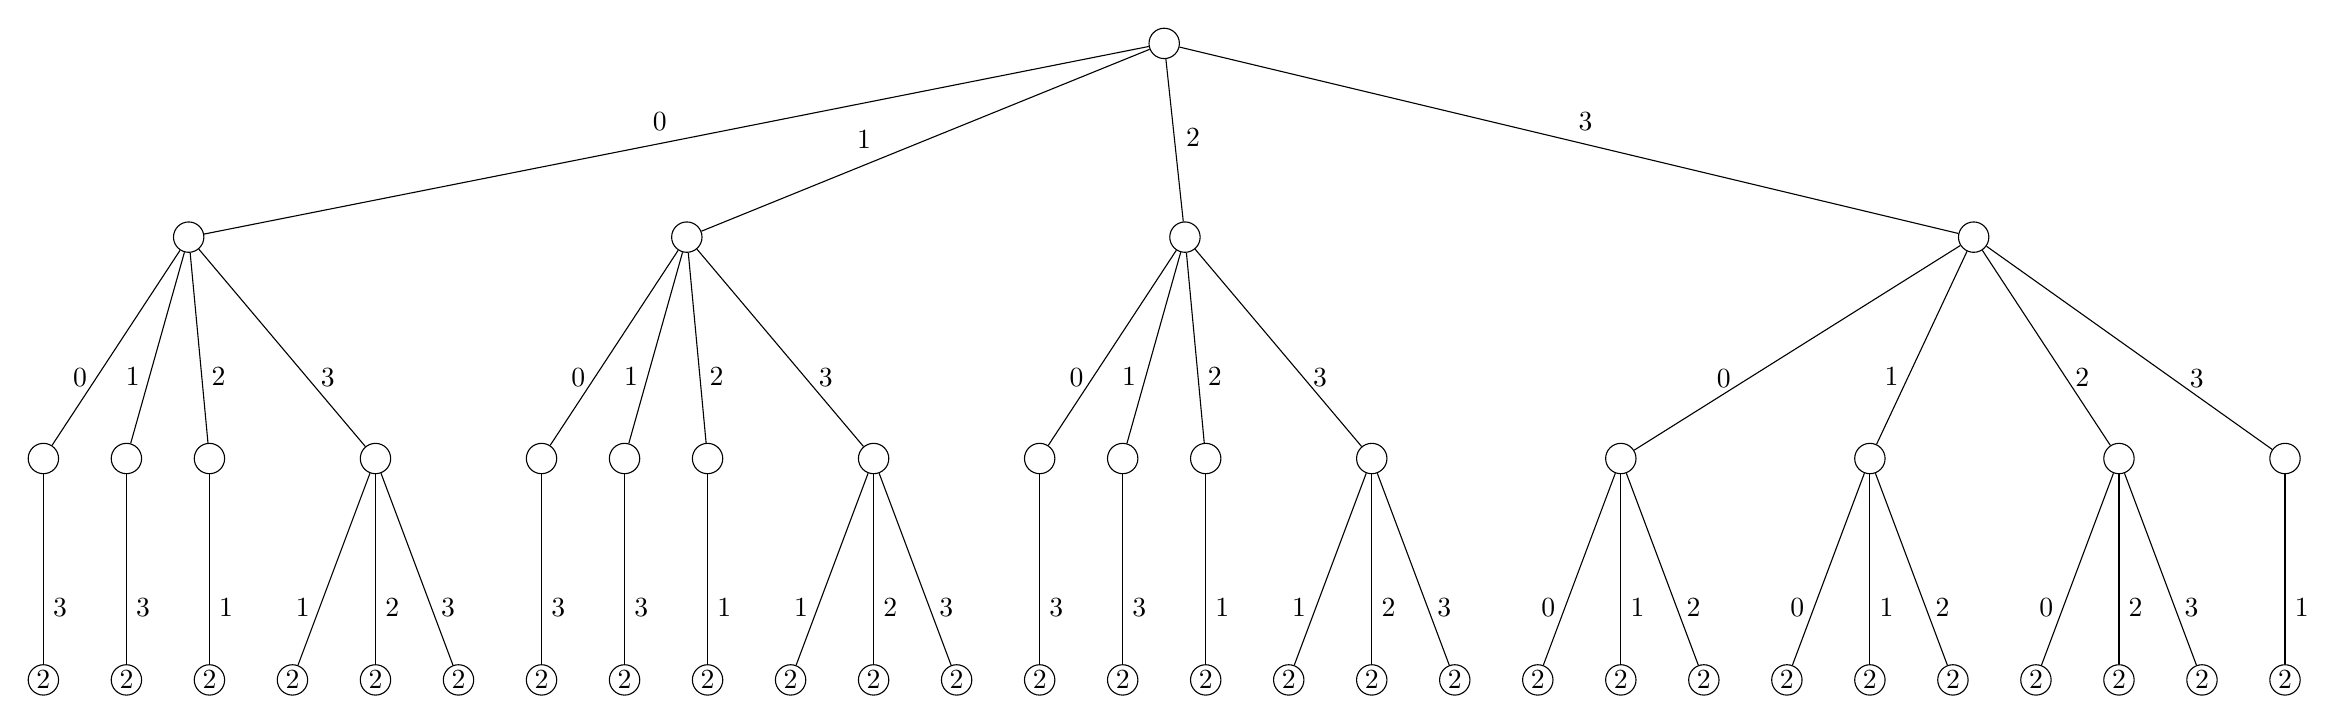
\begin{tikzpicture}[grow=down, edge from parent/.style={draw, -latex}]
    \label{fig:sea-automaton}

    \node at (0pt, 0pt) (S) [shape=circle,draw,inner sep=1pt] {\phantom{0}};

    \node at (-352.5pt, -70pt) (S0) [shape=circle,draw,inner sep=1pt] {\phantom{0}};
    \node at (-172.5pt, -70pt) (S1) [shape=circle,draw,inner sep=1pt] {\phantom{0}};
    \node at (7.5pt,    -70pt) (S2) [shape=circle,draw,inner sep=1pt] {\phantom{0}};
    \node at (292.5pt,  -70pt) (S3) [shape=circle,draw,inner sep=1pt] {\phantom{0}};

    \node at (-405pt, -150pt) (S00) [shape=circle,draw,inner sep=1pt] {\phantom{0}};
    \node at (-375pt, -150pt) (S01) [shape=circle,draw,inner sep=1pt] {\phantom{0}};
    \node at (-345pt, -150pt) (S02) [shape=circle,draw,inner sep=1pt] {\phantom{0}};
    \node at (-285pt, -150pt) (S03) [shape=circle,draw,inner sep=1pt] {\phantom{0}};

    \node at (-225pt, -150pt) (S10) [shape=circle,draw,inner sep=1pt] {\phantom{0}};
    \node at (-195pt, -150pt) (S11) [shape=circle,draw,inner sep=1pt] {\phantom{0}};
    \node at (-165pt, -150pt) (S12) [shape=circle,draw,inner sep=1pt] {\phantom{0}};
    \node at (-105pt, -150pt) (S13) [shape=circle,draw,inner sep=1pt] {\phantom{0}};

    \node at (-45pt, -150pt) (S20) [shape=circle,draw,inner sep=1pt] {\phantom{0}};
    \node at (-15pt, -150pt) (S21) [shape=circle,draw,inner sep=1pt] {\phantom{0}};
    \node at (15pt,  -150pt) (S22) [shape=circle,draw,inner sep=1pt] {\phantom{0}};
    \node at (75pt,  -150pt) (S23) [shape=circle,draw,inner sep=1pt] {\phantom{0}};

    \node at (165pt, -150pt) (S30) [shape=circle,draw,inner sep=1pt] {\phantom{0}};
    \node at (255pt, -150pt) (S31) [shape=circle,draw,inner sep=1pt] {\phantom{0}};
    \node at (345pt, -150pt) (S32) [shape=circle,draw,inner sep=1pt] {\phantom{0}};
    \node at (405pt, -150pt) (S33) [shape=circle,draw,inner sep=1pt] {\phantom{0}};

    \node at (-405pt, -230pt) (F00_3) [shape=circle,draw,inner sep=1pt] {2};
    \node at (-375pt, -230pt) (F01_3) [shape=circle,draw,inner sep=1pt] {2};
    \node at (-345pt, -230pt) (F02_1) [shape=circle,draw,inner sep=1pt] {2};
    \node at (-315pt, -230pt) (F03_1) [shape=circle,draw,inner sep=1pt] {2};
    \node at (-285pt, -230pt) (F03_2) [shape=circle,draw,inner sep=1pt] {2};
    \node at (-255pt, -230pt) (F03_3) [shape=circle,draw,inner sep=1pt] {2};

    \node at (-225pt, -230pt) (F10_3) [shape=circle,draw,inner sep=1pt] {2};
    \node at (-195pt, -230pt) (F11_3) [shape=circle,draw,inner sep=1pt] {2};
    \node at (-165pt, -230pt) (F12_1) [shape=circle,draw,inner sep=1pt] {2};
    \node at (-135pt, -230pt) (F13_1) [shape=circle,draw,inner sep=1pt] {2};
    \node at (-105pt, -230pt) (F13_2) [shape=circle,draw,inner sep=1pt] {2};
    \node at (-75pt,  -230pt) (F13_3) [shape=circle,draw,inner sep=1pt] {2};

    \node at (-45pt,  -230pt) (F20_3) [shape=circle,draw,inner sep=1pt] {2};
    \node at (-15pt,  -230pt) (F21_3) [shape=circle,draw,inner sep=1pt] {2};
    \node at (15pt,   -230pt) (F22_1) [shape=circle,draw,inner sep=1pt] {2};
    \node at (45pt,   -230pt) (F23_1) [shape=circle,draw,inner sep=1pt] {2};
    \node at (75pt,   -230pt) (F23_2) [shape=circle,draw,inner sep=1pt] {2};
    \node at (105pt,  -230pt) (F23_3) [shape=circle,draw,inner sep=1pt] {2};

    \node at (135pt,  -230pt) (F30_0) [shape=circle,draw,inner sep=1pt] {2};
    \node at (165pt,  -230pt) (F30_1) [shape=circle,draw,inner sep=1pt] {2};
    \node at (195pt,  -230pt) (F30_2) [shape=circle,draw,inner sep=1pt] {2};
    \node at (225pt,  -230pt) (F31_0) [shape=circle,draw,inner sep=1pt] {2};
    \node at (255pt,  -230pt) (F31_1) [shape=circle,draw,inner sep=1pt] {2};
    \node at (285pt,  -230pt) (F31_2) [shape=circle,draw,inner sep=1pt] {2};
    \node at (315pt,  -230pt) (F32_0) [shape=circle,draw,inner sep=1pt] {2};
    \node at (345pt,  -230pt) (F32_2) [shape=circle,draw,inner sep=1pt] {2};
    \node at (375pt,  -230pt) (F32_3) [shape=circle,draw,inner sep=1pt] {2};
    \node at (405pt,  -230pt) (F33_1) [shape=circle,draw,inner sep=1pt] {2};

    \path[draw] (S) -- (S0) node [midway, above left, font=\normalsize] {0};
    \path[draw] (S) -- (S1) node [pos=0.6, above left, font=\normalsize] {1};
    \path[draw] (S) -- (S2) node [pos=0.6, above right, font=\normalsize] {2};
    \path[draw] (S) -- (S3) node [midway, above right, font=\normalsize] {3};

    \path[draw] (S0) -- (S00) node [pos=0.65, left, font=\normalsize] {0};
    \path[draw] (S0) -- (S01) node [pos=0.65, left, font=\normalsize] {1};
    \path[draw] (S0) -- (S02) node [pos=0.65, right, font=\normalsize] {2};
    \path[draw] (S0) -- (S03) node [pos=0.65, xshift=0.5mm, right, font=\normalsize] {3};

    \path[draw] (S1) -- (S10) node [pos=0.65, left, font=\normalsize] {0};
    \path[draw] (S1) -- (S11) node [pos=0.65, left, font=\normalsize] {1};
    \path[draw] (S1) -- (S12) node [pos=0.65, right, font=\normalsize] {2};
    \path[draw] (S1) -- (S13) node [pos=0.65, xshift=0.5mm, right, font=\normalsize] {3};

    \path[draw] (S2) -- (S20) node [pos=0.65, left, font=\normalsize] {0};
    \path[draw] (S2) -- (S21) node [pos=0.65, left, font=\normalsize] {1};
    \path[draw] (S2) -- (S22) node [pos=0.65, right, font=\normalsize] {2};
    \path[draw] (S2) -- (S23) node [pos=0.65, right] {3};

    \path[draw] (S3) -- (S30) node [pos=0.65, xshift=-1mm, left, font=\normalsize] {0};
    \path[draw] (S3) -- (S31) node [pos=0.65, left, font=\normalsize] {1};
    \path[draw] (S3) -- (S32) node [pos=0.65, right, font=\normalsize] {2};
    \path[draw] (S3) -- (S33) node [pos=0.65, xshift=1mm, right] {3};

    \path[draw] (S00) -- (F00_3) node [pos=0.7, right, font=\normalsize] {3};
    \path[draw] (S01) -- (F01_3) node [pos=0.7, right, font=\normalsize] {3};
    \path[draw] (S02) -- (F02_1) node [pos=0.7, right, font=\normalsize] {1};
    \path[draw] (S03) -- (F03_1) node [pos=0.7, left, font=\normalsize] {1};
    \path[draw] (S03) -- (F03_2) node [pos=0.7, right, font=\normalsize] {2};
    \path[draw] (S03) -- (F03_3) node [pos=0.7, right, font=\normalsize] {3};

    \path[draw] (S10) -- (F10_3) node [pos=0.7, right, font=\normalsize] {3};
    \path[draw] (S11) -- (F11_3) node [pos=0.7, right, font=\normalsize] {3};
    \path[draw] (S12) -- (F12_1) node [pos=0.7, right, font=\normalsize] {1};
    \path[draw] (S13) -- (F13_1) node [pos=0.7, left, font=\normalsize] {1};
    \path[draw] (S13) -- (F13_2) node [pos=0.7, right, font=\normalsize] {2};
    \path[draw] (S13) -- (F13_3) node [pos=0.7, right, font=\normalsize] {3};

    \path[draw] (S20) -- (F20_3) node [pos=0.7, right, font=\normalsize] {3};
    \path[draw] (S21) -- (F21_3) node [pos=0.7, right, font=\normalsize] {3};
    \path[draw] (S22) -- (F22_1) node [pos=0.7, right, font=\normalsize] {1};
    \path[draw] (S23) -- (F23_1) node [pos=0.7, left, font=\normalsize] {1};
    \path[draw] (S23) -- (F23_2) node [pos=0.7, right, font=\normalsize] {2};
    \path[draw] (S23) -- (F23_3) node [pos=0.7, right, font=\normalsize] {3};

    \path[draw] (S30) -- (F30_0) node [pos=0.7, left, font=\normalsize] {0};
    \path[draw] (S30) -- (F30_1) node [pos=0.7, right, font=\normalsize] {1};
    \path[draw] (S30) -- (F30_2) node [pos=0.7, right, font=\normalsize] {2};

    \path[draw] (S31) -- (F31_0) node [pos=0.7, left, font=\normalsize] {0};
    \path[draw] (S31) -- (F31_1) node [pos=0.7, right, font=\normalsize] {1};
    \path[draw] (S31) -- (F31_2) node [pos=0.7, right, font=\normalsize] {2};

    \path[draw] (S32) -- (F32_0) node [pos=0.7, left, font=\normalsize] {0};
    \path[draw] (S32) -- (F32_2) node [pos=0.7, right, font=\normalsize] {2};
    \path[draw] (S32) -- (F32_3) node [pos=0.7, right, font=\normalsize] {3};

    \path[draw] (S33) -- (F33_1) node [pos=0.7, right, font=\normalsize] {1};

\end{tikzpicture}
}
\caption{Unreduced automaton representation of the SEA S-box DDT.}
\end{figure}

Applying the quaternary reduction rules to this structure removes the repetitive blocks. For instance, in the first level of the automaton, the transitions on symbols \texttt{0}, \texttt{1}, and \texttt{2} are grouped together because their corresponding sub-matrices share an identical structure, immediately sparing half the necessary storage. At the terminal level, only a single accept state is required to represent the differential value 2. The final reduced automaton, shown in Figure~\ref{fig:sea-reduced-automaton}, contains only 8 states, a substantial compression compared to the 64 cells of the original matrix. The function table for $f_{D}$ now contains a single entry mapping the string $\texttt{003}$, corresponding to the only accept state, to the value 2.

\begin{figure}[ht]
\centering
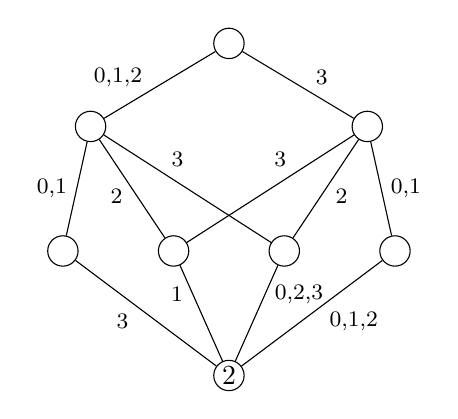
\begin{tikzpicture}[grow=down, level distance=50pt, edge from parent/.style={draw, -latex}]
    \label{fig:sea-reduced-automaton}

    \node (S) [shape=circle,draw,inner sep=1pt] {\phantom{0}};

    \node at (-50pt, -30pt) (S0) [shape=circle,draw,inner sep=1pt] {\phantom{0}};
    \node at (50pt, -30pt) (S3) [shape=circle,draw,inner sep=1pt] {\phantom{0}};
    
    \node at (-60pt, -75pt) (S00) [shape=circle,draw,inner sep=1pt] {\phantom{0}}; % 0002
    \node at (-20pt, -75pt) (S02) [shape=circle,draw,inner sep=1pt] {\phantom{0}}; % 0200
    \node at (20pt, -75pt) (S03) [shape=circle,draw,inner sep=1pt] {\phantom{0}}; % 2022
    \node at (60pt, -75pt) (S30) [shape=circle,draw,inner sep=1pt] {\phantom{0}}; % 2220

    \node at (0pt, -120pt) (F2) [shape=circle,draw,inner sep=1pt] {2};

    \path[draw] (S) -- (S0) node [midway, left, xshift=-1mm, yshift=1mm, font=\footnotesize] {0,1,2};
    \path[draw] (S) -- (S3) node [midway, right, xshift=1mm, yshift=1mm, font=\footnotesize] {3};

    \path[draw] (S0) -- (S00) node [midway, left, font=\footnotesize] {0,1};
    \path[draw] (S0) -- (S02) node [midway, left, yshift=-1mm, font=\footnotesize] {2};
    \path[draw] (S0) -- (S03) node [pos=0.3, right, xshift=1mm, yshift=1mm, font=\footnotesize] {3};
    \path[draw] (S3) -- (S30) node [midway, right, font=\footnotesize] {0,1};
    \path[draw] (S3) -- (S03) node [midway, right, yshift=-1mm, font=\footnotesize] {2};
    \path[draw] (S3) -- (S02) node [pos=0.3, left, xshift=-1mm, yshift=1mm, font=\footnotesize] {3};
    

    \path[draw] (S00) -- (F2) node [midway, left, xshift=-1mm, yshift=-1mm, font=\footnotesize] {3};
    \path[draw] (S02) -- (F2) node [pos=0.3, left, font=\footnotesize] {1};
    \path[draw] (S03) -- (F2) node [pos=0.3, right, font=\footnotesize] {0,2,3};
    \path[draw] (S30) -- (F2) node [midway, right, xshift=1mm, yshift=-1mm, font=\footnotesize] {0,1,2};

\end{tikzpicture}
\caption{SEA reduced automaton.}
\end{figure}


